\documentclass[10pt,twoside]{article}
\usepackage[utf8]{inputenc}
\usepackage{amsmath}
\usepackage{amsfonts}
\usepackage{amssymb}
\usepackage[spanish,es-noshorthands]{babel}
\usepackage[T1]{fontenc}
\usepackage{lmodern}
\usepackage{graphicx,hyperref}
\usepackage{tikz,pgf}
\usepackage{multicol}
\usepackage{subfig}
\usepackage[papersize={6.5in,8.5in},width=5.5in,height=7in]{geometry}
\usepackage{fancyhdr}
\pagestyle{fancy}
\fancyhead[LE]{
\includegraphics[height=12pt]{Images/logo-colegio.png} Aritmética $6^{\circ}$}
\fancyhead[RE]{}
\fancyhead[RO]{\textit{Germ\'an Avenda\~no Ram\'irez, Lic. U.D., M.Sc. U.N.}}
\fancyhead[LO]{}

\author{Germ\'an Avenda\~no Ram\'irez, Lic. U.D., M.Sc. U.N.}
\title{\begin{minipage}{.2\textwidth}

\includegraphics[height=1.75cm]{Images/logo-colegio.png}\end{minipage}
\begin{minipage}{.55\textwidth}
\begin{center}
Taller 12, Números primos  \\
Aritmética $6^{\circ}$
\end{center}
\end{minipage}\hfill
\begin{minipage}{.2\textwidth}

\includegraphics[height=1.75cm]{Images/logo-sed.png} 
\end{minipage}}
\date{}
\begin{document}
\maketitle
Nombre: \hrulefill Curso: \underline{\hspace*{44pt}} Fecha: \underline{\hspace*{2.5cm}}\\
\begin{enumerate}
 \item Construya los diagramas de árbol, para hallar los divisores de 36, de 100 y de 144
 \begin{enumerate}
  \item ¿Cuántos divisores tiene cada número?
  \item ¿Los divisores de un número son menores que él? ¿Por qué?
 \end{enumerate}
\item Sonia prepara para la venta, galletas de coco. Cada grupo de 24 galletas las empaca en cajas rectangulares, de manera que no sobren ni falten. ¿Cuáles son las posibles distribuciones que pueden hacer en las cajas para guardar las galletas?
\begin{center}
 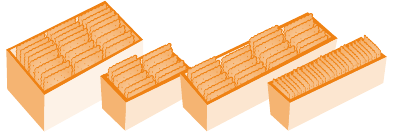
\includegraphics{./Images/galletas.png}
 % galletas.png: 393x133 pixel, 96dpi, 10.40x3.52 cm, bb=0 0 295 100
\end{center}
\item  ¿Cuáles serían las posibles distribuciones si las cajas contienen
40 galletas? Represéntalas
\end{enumerate}
\section*{¿Conoces los números primos?}
\subsection*{Lo que sé}
Resuelve individualmente

\begin{minipage}[]{.55\textwidth}
En el criadero de reptiles también tienen lagartos de diferentes especies. Uno de ellas es el lagarto arlequín que pone entre 30 y 40 huevos de forma alargada.

Una mañana Juan recogió huevos de dos hembras de esta especie. Una de ellas tenía 36 huevos y la otra 37. Cada grupo de huevos debía acomodarse en una cubeta como la de la figura. 
\end{minipage} \hfill
\begin{minipage}{.35\textwidth}
 \begin{center}
 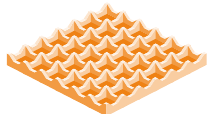
\includegraphics{./Images/cubeta.png}
 % cubeta.png: 211x114 pixel, 96dpi, 5.58x3.02 cm, bb=0 0 158 85
\end{center}
\end{minipage}
\begin{itemize}
 \item ¿Qué grupo de huevos puede acomodar Juan en las cubetas,
sin que le sobren? Explica
\end{itemize}
\subsection*{Aprende algo nuevo}

\end{document}
